\section{Satisfiability}
\label{sec:satisfiability}

This part of the project is aimed at solving the BWP using the satisfiability
paradigm, that is, by constructing a Boolean formula in Conjunctive Normal Form
(CNF), using a number of Boolean variables, and then solving it. The solution
is a truth assignment to the variables. The way this solution is obtained is
by means of a SAT solver.

\hfill

This time, this paradigm has mostly only disadvantages: not only we cannot find
an optimal solution directly just by finding a truth assignment to the variables,
but also the ``language'' is less expressive, or, rather, more rigid since it
only allows Boolean clauses in CNF than the one used in Constraint or Linear
Programming. However, the constraints and variables that have to be imposed
are exactly the same as the ones formalised in section \ref{sec:modelling} and,
as will be explained in the coming sections, optimality can be reached using
fairly simple methods.

\hfill

By less expressive we mean the following: take, for example, the constraint
\ref{constr:box-placed} formalised in section \ref{sec:modelling:constraints}.
This constraint formalised the idea that each box has to have its
top-left corner assigned to exactly one cell, and, given the Boolean variables
detailed in \ref{var:box-corner} for each cell on the roll for a certain box, we
only had to add up all the variables and impose that the sum be equal to 1.
This was implemented in sections \ref{sec:constraint-programming} and
\ref{sec:linear-programming} following equation \ref{eq:constraint:all-boxes-used}
literally. This time we can not do this. In Boolean satisfiability this can be seen
as ``given $n$ Boolean variables, exactly one of the $n$ variables $x_1,\cdots,x_n$
has to be true''. Encoding this constraint requires two types of constraints:
``at least one'' and ``at most one''. If we manage to encode them using two Boolean
expressions in CNF each, the conjunction of the two will give us the ``exactly one''
constraint:
\begin{itemize}
	\item At least one: given variables $x_1,\cdots,x_n$ at least
	one of them must be true. This is straightforward, we only need
	to add the following clause to the Boolean formula:
	\begin{equation}
	\label{eq:cnf:at-least-one}
	x_1 \vee x_2 \vee \cdots \vee x_n
	\end{equation}
	Since all clauses of the formula have to evaluate to true to make
	it satisfiable then at least one of the variables $x_i$ must be set to true.
	
	\item At most one: given variables $x_1,\cdots,x_n$ at most
	one of them must be true. This is the most difficult constraint
	to implement using a Boolean formula in CNF. To begin with, there
	are different ways to encode this constraint. Here are listed
	three of them:
	\begin{enumerate}
		\item Quadratic encoding ($\mathcal{Q}$): the simplest of the
		encodings, we only have to add the clauses
		\begin{equation}
		\label{eq:cnf:at-most-one:quad}
		\mathcal{Q}(x_1,\cdots, x_n) =
		\bigvee_{1 \le i < j \le n} (\overline{x_i}\vee\overline{x_j})
		\end{equation}
		which will produce $\binom{n}{2} = O(n^2)$ clauses.
		
		\item Logarithmic encoding ($\mathcal{L}$): this encoding uses
		$m = \lceil \log{n} \rceil$ extra variables to encode the
		intended meaning. Given $n$ variables, introduce variables
		$y_0,\cdots,y_{m-1}$ and add the following clauses:
		\begin{equation}
		\label{eq:cnf:at-most-one:log}
		\mathcal{L}(x_1,\cdots, x_n) = 
		\bigwedge_{i=1}^n
		\left(\bigwedge_{j} (\overline{x_i} \vee y_j) \right)
		\wedge
		\left(\bigwedge_{k} (\overline{x_i} \vee \overline{y_k}) \right)
		\end{equation}
		for the bits $j$ set to 1 in the binary representation of $i$ and
		for the bits $k$ set to 0 in the binary representation of $i$, respectively.
		Since for each variable $O(\log{n})$ clauses are added, the logarithmic
		encoding produces in total $O(n\log{n})$ clauses.
		
		\item Heule encoding ($\mathcal{H}$): this encoding is based on
		the quadratic encoding. The set of clauses produced $\mathcal{H}(x_1,\cdots, x_n)$
		is defined with the following recurrence:
		\begin{equation}
		\label{eq:cnf:at-most-one:heule}
		\mathcal{H}(x_1,\cdots, x_n) =
		\left\{
		\begin{array}{l l}
		\mathcal{Q}(x_1,\cdots, x_n) & \text{ if } n \le 3 \\
		\mathcal{Q}(x_1,x_2,y) \wedge \mathcal{H}(x_3,\cdots, x_n, \overline{y}) & \text{ otherwise}
		\end{array}
		\right.
		\end{equation}
		where $y$ denotes a new variable that was not used before.
	\end{enumerate}
\end{itemize}

The performance of the SAT solver will depend largely on the encoding chosen for
constraints of type ``at most one''. Further details are given in section
\ref{sec:benchmarking:satisfiability}.

\subsection{Implementation}
\label{sec:satisfiability:implementation}

This time we did not need to implement any array of variables, since
we only have to output the clauses into a file that will be used by a
SAT solver. However, each variable needs an identifier (starting at 1).
Generating these identifiers is done via the following functions:

\begin{enumerate}
	\item Variables in \ref{var:box-cell} ($C_{b,x,y}$):
    
	{\NOINDENT \begin{lstlisting}
	// 0 <= b < N, 0 <= x < W, 0 <= y < L
	int C(int b, int x, int y) {
		return nXvars + 1 + b*W*L + y*W + x;
	}
	\end{lstlisting}}
    
	\item Variables in \ref{var:box-corner} ($X_{b,x,y}$):
    
	{\NOINDENT \begin{lstlisting}
	// 0 <= b < N, 0 <= x < W, 0 <= y < L
	int X(int b, int x, int y) {
		return 1 + b*W*L + y*W + x;
	}
	\end{lstlisting}}
    
	\item Variables in \ref{var:box-rotated} ($R_b$):
    
	{\NOINDENT \begin{lstlisting}
	// 0 <= b < N
	int R(int b) {
		return nXvars + nCvars + 1 + b;
	}
	\end{lstlisting}}
\end{enumerate}

The variables $nXVars$, $nCvars$ and $nRvars$ store the amount of
variables for $X_{b,i,j}$, $C_{b,i,j}$ and $R_b$ respectively. The
amounts of each type of variables is given at the end of section
\ref{sec:modelling:variables}. Variables $W$ and $L$ store the
roll's width and length, respectively.

\hfill

While keeping in mind the implementation of these functions, and
assuming the existence of a class \textbf{clause} which represents a list
of literals, and the existence of an object \textbf{CE} which is capable
of encodign the ``at least/most one'' constraints in the three
different ways detailed above ($\mathcal{Q}$, $\mathcal{L}$, and
$\mathcal{H}$), the constraints in section \ref{sec:modelling:constraints}
have been implemented as follows:

\begin{enumerate}
	\item All boxes must be in the solution (constraint formalised in
	\ref{constr:box-placed}, equation \ref{eq:constraint:all-boxes-used}),
	also read as ``assign a top-left corner to each box''. This has been
	slightly modified: the first for loop forces the box with index 0 (the first
	that is read from the input file) to be placed, unconditionally, on the upper-left
	quadrant of the roll. This model-independent constraint will produce less
	clauses which we expect will translate into an increase of the efficiency while
	mantaining correctness.
    
	{\NOINDENT \begin{lstlisting}
	clause cl0;
	for (length y = 0; y < L/2; ++y) {
		for (width x = 0; x < W/2; ++x) {
			cl0 += X(0,x,y);
		}
	}
	CE.exactly_one(cl0, out);
	for (size_t b = 1; b < N; ++b) {
		clause cl;
		for (length y = 0; y < L; ++y) {
			for (width x = 0; x < W; ++x) {
				cl += X(b,x,y);
			}
		}
		CE.exactly_one(cl, out);
	}
	\end{lstlisting}}
    
	\item Boxes cannot overlap (constraint formalised in
	\ref{constr:no-overlap}, constraint \ref{eq:constraint:one-box-cell}).
    
	{\NOINDENT \begin{lstlisting}
	for (length y = 0; y < L; ++y) {
		for (width x = 0; x < W; ++x) {
			clause cl;
			for (size_t b = 0; b < N; ++b) {
				cl += C(b,x,y);
			}
			CE.amo(cl, out);
		}
	}
	\end{lstlisting}}
    
	\item Depending on their rotation, boxes occupy certain cells of the roll
	(constraint formalised in \ref{constr:box-rot-span}). For those cells $(x,y)$ within
	bounds for $b$-th box:

	\begin{itemize}
		\item For square boxes (constraint \ref{eq:span-cells:square-boxes}):
		{\NOINDENT \begin{lstlisting}
		for (length i = y; i <= y + b_length - 1; ++i) {
			for (width j = x; j <= x + b_width - 1; ++j) {
				out << -X(b,x,y) << " " << C(b,j,i) << " 0" << endl;
			}
		}
		out << -R(b) << " 0" << endl;
		\end{lstlisting}}
		
		\item For rectangular boxes (constraints \ref{eq:span-cells:rectangular-boxes:0} and
		\ref{eq:span-cells:rectangular-boxes:1}):
		{\NOINDENT \begin{lstlisting}
		for (length i = y; i <= y + b_length - 1; ++i) {
			for (width j = x; j <= x + b_width - 1; ++j) {
				out << R(b) << " " << -X(b,x,y) << " " << C(b,j,i) << " 0" << endl;
			}
		}
		\end{lstlisting}}
		{\NOINDENT \begin{lstlisting}
		for (length i = y; i <= y + b_width - 1; ++i) {
			for (width j = x; j <= x + b_length - 1; ++j) {
				out << -R(b) << " " << -X(b,x,y) << " " << C(b,j,i) << " 0" << endl;
			}
		}
		\end{lstlisting}}
	\end{itemize}
    
	\item Depending on their rotation, boxes cannot occupy certain cells of the
	roll (constraint formalised in \ref{constr:box-forbid}). For those cells $(x,y)$
	out of bounds for $b$-th box:
    
	\begin{itemize}
		\item For square boxes (constraint \ref{eq:forbid-span-cells:square-boxes}):
		{\NOINDENT \begin{lstlisting}
		out << -X(b,x,y) << " 0" << endl;
		\end{lstlisting}}
		
		\item For rectangular boxes (constraints \ref{eq:forbid-span-cells:rectangular-boxes:0}
		and \ref{eq:forbid-span-cells:rectangular-boxes:1}):
		{\NOINDENT \begin{lstlisting}
		out << R(b) << " " << -X(b,x,y) << " 0" << endl;
		\end{lstlisting}}
		{\NOINDENT \begin{lstlisting}
		out << -R(b) << " " << -X(b,x,y) << " 0" << endl;
		\end{lstlisting}}
	\end{itemize}
    
\end{enumerate}

Notice that all the clauses produced by the last constraint are clauses with at most
two literals (Horn clauses). Some other constraints are also implemented using Horn clauses.
Furhermore, any of the encodings used for the ``at most one'' constraints are also Horn
clauses. This allows for easy propagation for the SAT solver that will be used. However,
the problem cannot be solved in polynomial time since some of the clauses have 3 literals.

\subsection{Finding the optimum solution}
\label{sec:satisfiability:optimum}

Likewise the Constraint Programming paradigm, Satisfiability is not defined to solve
optimisation problems either. However, we can use a SAT solver as a black box to find
optimal solutions. To achieve this, the ideas explained in section
\ref{sec:constraint-programming:optimum} will be applied similarly within a framework
that consists of three independent modules: the clause generator,
the SAT solver, and the solution generator. The first will generate the necessary
clauses in CNF for a given instance of the Box Wrapping Problem, which will be passed
on to the SAT solver, which in turn will compute a truth assignment (or decide that the
Boolean formula is unsatisfiable). If the formula is satisfiable then the solution
generator will process this truth assignment and build a solution, that is, find
the position of each top-left and bottom-right corners for each box. Now, this
solution generator returns the length that was used and sends it to the clause generator
which will compute the minimum between the length's upper bound (using equation
\ref{eq:upper-bound-L}) and this value (minus 1). Basically, the ideas behind equation
\ref{eq:upper-bound-L:better} are applied so as to force the SAT solver find a solution
with a shorter roll length. This process is applied until the SAT solver decides that
the Boolean formula generated is unsatisfiable, which implies that optimality was reached.
See figure \ref{fig:satisfiability:framework} for a graphical representation of this
process. Therefore, the optimal value of the roll's length $L$ is such that the Boolean
formula produced is satisfiable, but the one produced with $L - 1$ is unsatisfiable.

\begin{figure}[H]
	\centering
	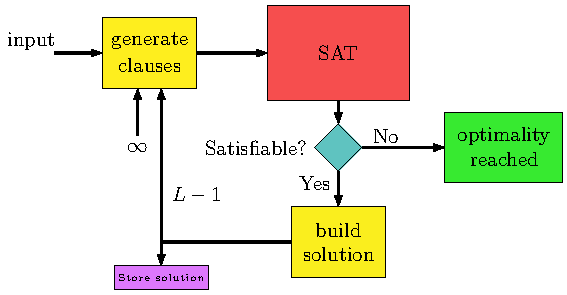
\includegraphics{satisfiability/framework}
	\centeredcaption{Finding an optimal solution using a SAT solver. The initial
	value of the length used in equation \ref{eq:upper-bound-L:better} is $\infty$.}
	\label{fig:satisfiability:framework}
\end{figure}

Other methods could have been used. For example, binary search could have been applied.
However, deciding whether a Boolean formula is satisfiable (and computing a
truth value in case it is) is far easier than concluding unsatisfiablity. This way
we avoid sending values of $L$ that will certainly lead to producing an unsatisfiable
formula hence facing the challenge of deciding unsatisfiability only once (for that
one value of $L$ that will certainly define the optimal value of the roll's length).

\subsection{Compilation and execution}
\label{sec:satisfiability:compilation-execution}

In order to compile this part of the project, while assuming that we are at the
root directory of the project, one should issue the following commands:
\begin{lstlisting}[language=bash]
~/box-wrapping$ cd SAT/build-rules
~/box-wrapping/SAT/build-rules$ make -f Makefile release
~/box-wrapping/SAT/build-rules$ cd ..
~/box-wrapping/SAT$ cd build-release
\end{lstlisting}

This will generate two executable files: \textit{clause-generator} and
\textit{solution-generator}. The former generates the clauses and the latter
takes the solution of the SAT solver and builds the solution. The clauses generated
have been tested only on the \textbf{lingeling} SAT solver (see \cite{lingeling}).
Moreover, the file generated has to be reversed. The solution generated by the solver
has to be processed so that only the truth assignment is left on the file (the numeric
values representing this truth assignment: if variable $x_1$ is assigned to true
then the numerical value is ``$1$''. If it is assigned to false then it is ``$-1$'').

\hfill

The clause generator has been designed to support two ways of solving an instance:
when we allow the boxes to rotate, and when we do not. Moreover, the three types of
encodings ($\mathcal{Q}$, $\mathcal{L}$, and $\mathcal{H}$) explained at the beginning
of this section. In figures \ref{fig:satisfiability:clause-generator} and
\ref{fig:satisfiability:solution-generator} are shown two examples of usage of these
modules.

\begin{figure}[H]
\centering
\begin{lstlisting}[language=bash,basicstyle=\centering]
$ ./clause-generator -i bwp_3_3_1.in -o bwp.cnf.rev \
					 --solver rotate --amo-encoder heule --max-L 1
\end{lstlisting}
\centeredcaption{An example of how to use the \textit{clause-generator} module.}
\label{fig:satisfiability:clause-generator}
\end{figure}

\begin{figure}[H]
\centering
\begin{lstlisting}[language=bash,basicstyle=\centering]
$ ./solution-generator --boxes bwp_3_3_1.in --variables bwp.vars \
					   -o bwp_3_3_1.out --solver rotate --max-L 1
\end{lstlisting}
\centeredcaption{An example of how to use the \textit{solution-generator} module.}
\label{fig:satisfiability:solution-generator}
\end{figure}

Since the process of specifying the parameters correctly, while preprocessing the
files for and produced by the SAT solver, is rather cumbersome, the process depicted
in figure \ref{fig:satisfiability:framework} is governed by the script \textit{exe-SAT.sh}
in the \textit{box-wrapping/SAT/} directory. It requires the file with the description
of the instance, the name of the file containig its solution, what solver should be
used, and, optionally, what encoder has to be used for the ``at most one'' constraints
($\mathcal{Q}$, $\mathcal{L}$, and $\mathcal{H}$), and two timeouts, one for the whole
script and another for the SAT solver. An example can be seen in figure
\ref{fig:satisfiability:gov-script}.

\begin{figure}[H]
\centering
\begin{lstlisting}[language=bash,basicstyle=\centering]
$ ./exe-SAT.sh	-i=bwp_3_3_1.in -o=bwp_3_3_1.out \
				--solver=rotate	--amo-encoder=logarithmic
\end{lstlisting}
\centeredcaption{An example of how to use the \textit{exe-SAT.sh} script.}
\label{fig:satisfiability:gov-script}
\end{figure}

The output of this script for the example in figure \ref{fig:satisfiability:gov-script}
is the following:
\begin{figure}[H]
\centering
{\scriptsize
\begin{BVerbatim}
    Try max length: 999999      |    Try max length: 2          |    Try max length: 1
        At iteration: 0         |        At iteration: 1        |        At iteration: 2
      | W                       |      | W                      |      | W
    L | 0 1 2                   |    L | 0 1 2                  |    L | 0 1 2 
    ----------                  |    ----------                 |    ----------
    0 | 1 . .                   |    0 | . 3 2                  |    0 | 3 2 1 
    1 | . 3 .                   |    1 | 1 . .                  |    
    2 | . . 2                   |                               |    Boxes' corners:      (w,l)
                                |    Boxes' corners:      (w,l) |        Box 1 is at 
    Boxes' corners:      (w,l)  |        Box 1 is at            |            top left     (2,0)
        Box 1 is at             |            top left     (0,1) |            bottom right (2,0)
            top left     (0,0)  |            bottom right (0,1) |    
            bottom right (0,0)  |                               |        Box 2 is at 
                                |        Box 2 is at            |            top left     (1,0)
        Box 2 is at             |            top left     (2,0) |            bottom right (1,0)
            top left     (2,2)  |            bottom right (2,0) |    
            bottom right (2,2)  |                               |        Box 3 is at 
                                |        Box 3 is at            |            top left     (0,0)
        Box 3 is at             |            top left     (1,0) |            bottom right (0,0)
            top left     (1,1)  |            bottom right (1,0) |    
            bottom right (1,1)  |                               |        Roll length used: 1
                                |        Roll length used: 2    |
        Roll length used: 3     |                               |    Try max length: 0
                                |                               |        At iteration: 3
                                |                               |        lingeling determined unsatisfiability
                                |                               |        of the Boolean formula
                                |                               |           Optimality reached!
\end{BVerbatim}
}
\centeredcaption{Edited output of the script \textit{exe-SAT.sh} using the parameters of the
example in figure \ref{fig:satisfiability:gov-script}.}
\label{fig:satisfiability:gov-script:result}
\end{figure}
